\documentclass[a4paper,12pt]{article}
%%%%%%%%%%%%%%%%%%%%%%%%%%%%%%%%%%%%%%%%%%%%%%%%%%%%%%%%%%%
%%%%% 	pour le français et les accents 	      %%%%%
%%%%%%%%%%%%%%%%%%%%%%%%%%%%%%%%%%%%%%%%%%%%%%%%%%%%%%%%%%%
\usepackage[utf8]{inputenc}
\usepackage[french]{babel}
%%%%%%%%%%%%%%%%%%%%%%%%%%%%%%%%%%%%%%%%%%%%%%%%%%%%%%%%%%%
\usepackage[T1]{fontenc}
\usepackage{amsmath}
\usepackage{amssymb}
\usepackage[top=1.1in,bottom=1.5in]{geometry}
\usepackage{dsfont}       % for  \mathds and nice 0/1 functions
\usepackage{graphicx}     % for images and graphics
\usepackage{stmaryrd}     % for \llbrackets
\usepackage{color}
\usepackage{subeqnarray}
\usepackage{pdflscape}
\usepackage{multirow}
\usepackage{threeparttable}
\usepackage{booktabs}
%%%%%%%%%%%%%%%%%%%%%%%%%%%%%%%%%%%%%%%%%%%%%%%%%%%%%%%%%%%
%%%%% 	package pour les algorithmes		       %%%%%%%%
%%%%%%%%%%%%%%%%%%%%%%%%%%%%%%%%%%%%%%%%%%%%%%%%%%%%%%%%%%%
\usepackage{algpseudocode}
\usepackage{algpascal}
\usepackage{amsmath}
\usepackage[linesnumbered,ruled]{algorithm2e}
%%%%%%%%%%%%%%%%%%%%%%%%%%%%%%%%%%%%%%%%%%%%%%%%%%%%%%%%%%%
%%%%%   package pour les graphe                     %%%%%%%
%%%%%%%%%%%%%%%%%%%%%%%%%%%%%%%%%%%%%%%%%%%%%%%%%%%%%%%%%%%
\usepackage{pgf,tikz}
\usepackage{mathrsfs}
\usepackage[font={small,sf},labelfont=bf,format=hang,format=plain,width=0.8\textwidth,]{caption}
\usepackage[list=true]{subcaption}
\usetikzlibrary{arrows}
%%%%%%%%%%%%%%%%%%%%%%%%%%%%%%%%%%%%%%%%%%%%%%%%%%%%%%%%%%%
%%%%% 	pour des liens hypertextes  et du jpg  	    %%%%%%%
%%%%%%%%%%%%%%%%%%%%%%%%%%%%%%%%%%%%%%%%%%%%%%%%%%%%%%%%%%%
\usepackage[pdftex,a4paper,linkcolor=freeblue,citecolor=vertsombre,colorlinks=true,pagebackref,bookmarks=true, plainpages=true,urlcolor=freeblue]{hyperref}
%%%%%%%%%%%%%%%%%%%%%%%%%%%%%%%%%%%%%%%%%%%%%%%%%%%%%%%%%%%
%%%%%  		Couleurs			%%%%%%%%%%%
%%%%%%%%%%%%%%%%%%%%%%%%%%%%%%%%%%%%%%%%%%%%%%%%%%%%%%%%%%%
\definecolor{test}{rgb}{0.64,0.16,0.16}
\definecolor{vertsombre}{rgb}{0.00,0.57,0.1}
\definecolor{freeblue}{rgb}{0.25,0.41,0.88}
\definecolor{qqqqff}{rgb}{0.,0.,1.}
\definecolor{zzttqq}{rgb}{0.6,0.2,0.}
\definecolor{uuuuuu}{rgb}{0.26666666666666666,0.26666666666666666,0.26666666666666666}
\definecolor{xdxdff}{rgb}{0.49019607843137253,0.49019607843137253,1.}
\definecolor{cqcqcq}{rgb}{0.7529411764705882,0.7529411764705882,0.7529411764705882}
%%%%%%%%%%%%%%%%%%%%%%%%%%%%%%%%%%%%%%%%%%%%%%%%%%
%%%%%%		Début du document 	    %%%%%%
%%%%%%%%%%%%%%%%%%%%%%%%%%%%%%%%%%%%%%%%%%%%%%%%%%
\begin{document}
	\title{\vspace{-1.5cm}Polyomino Tilings and Exact Cover}
	\author{Ke WANG, Shiwen XIA}
	\maketitle
	\tableofcontents
	\newpage
	\section{Introduction}
	Un polyomino est une réunion connexe de carrés unitaires. Il existe 3 méthodes pour définir les polyominoes selon leur forme\cite{wikipedia}:
	\begin{description}
		\item[$\bullet$ fixé :] Des polyominoes sont considérés equivalents seulement s'ils diffèrent par la translation.
		\item[$\bullet$ à un seul côté :] Des polyominoes sont considérés equivalents s'ils diffèrent par la translation et la rotation dans le plan.
		\item[$\bullet$ libre :] Des polyominoes sont considérés equivalents s'ils diffèrent par n'import quelle transformation.
	\end{description}
	\par Le problème de \textit{Polyominoes tilings and exact cover} est NP-complet. Ce projet se consacre à trouver un algorithme et une efficace structure des données à énumérer les polyominoes d'une taille spécifique et puis résoudre le problème de \textbf{couverture exacte}.
	%%%%%%%%%%%%%%%%%%%%%%%%%%%%%%%%%%%%%%%%%%%%%%%%%%%%%%%%%%%%%%%%%%%%%%%%%%%%%%%%%%%%%%%%%%
	%%%%%%%%%%%%%%%%%%%%%%%%%%%%%%%%%%%%%%%%%%%%%%%%%%%%%%%%%%%%%%%%%%%%%%%%%%%%%%%%%%%%%%%%%%
	\section{Enumération des polyominoes}
	\par L'obstacle essentiel à l'énumération est d'éviter le double compte d'un même polyomino. À cet effet, il y a deux façons faisables. Une façon naïve est que nous générons tous les polyominoes possibles de toute façon, mais nous ne comptons que ceux qui sont différents et négligeons ceux qui sont déjà comptés. Une deuxième façon est d'améliorer l'algorithme de générateur de polyominoes afin qu'il ne génère que des polyominoes différents.
	\par Au niveau de structure des données, nous avons également deux stratégies. Nous pouvons stocker un polyomino, ainsi que ses informations caractéristiques chaque fois quand nous le trouvons adapté. Avec cette manière, nous pouvons nous enquérir facilement les informations utiles dans les questions suivantes, alors que nous risquons de perdre l'efficacité de mémoire. Différemment, nous pouvons calculer le nombre de polyominoes d'une taille spécifique sans les stocker. Cette stratégie serrait évidenment plus efficace mais pas assez convenable pour des questions suivantes.
	\par Dans cette section, nous montrerons ces deux algorithmes d'énumération et les deux structures des données correspondantes. Ensuite, nous les comparerons pour choisir une méthode pertinente à stocker les informations dont nous aurons besoin.
	%%%%%%%%%%%%%%%%%%%%%%%%%%%%%%%%%%%%%%%%%%%%%%%%%%%%%%%%%%%%%%%%%%%%%%%%%%%%%%%%%%%%%%%%%%
	\subsection{Algorithme Naïf}
	\par Pour générer un polyomino de taille \textit{N}, nous pouvons le considérer comme successeur d'un polyomino de taille \textit{N-1}. Chaque polyomino de taille \textit{N-1} a plusieurs cases \textit{attachables}, à savoir que le nouveau polyomino (taille \textit{N}) composé de ce polyomino (taille \textit{N-1}, appelé le prédécesseur) et la case attachée, qui est appelé un successeur, est également un polyomino \textit{légal}.
	\par Basé sur cette idée, un algorithme intuitif peut être exprimé par pseudo-code ci-dessous :
	\begin{algorithm}
		\SetKwInOut{Input}{Input}
		\SetKwInOut{Output}{Output}	
		\Input{Collection of all polyominoes of size \textit{N-1} : $\mathcal{P}(N-1)$}	
		\Output{Collection of all polyominoes of size \textit{N} : $\mathcal{P}(N)$}
		$\mathcal{P}(N) = \emptyset$\;
		\For{p $\leftarrow$ element of $\mathcal{P}(N-1)$}{
			$\mathcal{C}(p) \leftarrow$ all attachable cells of $p$ \;
			\For{c $\leftarrow$ cell in $\mathcal{C}(p)$}{
				$new\_p \leftarrow p \cup c$\;
				\If{$new\_p \not\in \mathcal{P}(N)$}{
					$\mathcal{P}(N):=\mathcal{P}(N)$ $\cup$ $new\_p$\;
				}
			}
		}
		\caption{A naive algorithm for \textit{task 2}}
		\label{algo:fixed count}
	\end{algorithm}
	\begin{figure}[h]
	\centering
	\begin{subfigure}[]{0.35\textwidth}
		\centering
		\begin{tikzpicture}[line cap=round,line join=round,>=triangle 45,x=0.5cm,y=0.5cm]
		\draw [line width=2.pt] (10.,6.)-- (18.,6.);
		\draw [line width=2.pt] (10.,8.)-- (18.,8.);
		\draw [line width=2.pt] (16.,10.)-- (16.,6.);
		\draw [line width=2.pt] (12.,4.)-- (12.,8.);
		\draw [line width=2.pt] (10.,8.)-- (10.,6.);
		\draw [line width=2.pt] (18.,8.)-- (18.,6.);
		\draw [line width=2.pt] (14.,4.)-- (14.,10.);
		\draw [line width=2.pt] (14.,10.)-- (16.,10.);
		\draw [line width=2.pt] (12.,4.)-- (14.,4.);
		\end{tikzpicture}
	\end{subfigure}
	\begin{subfigure}[]{0.18\textwidth}
		\centering
		$\Rightarrow$
	\end{subfigure}
	\begin{subfigure}[]{0.45\textwidth}
		\centering
		\begin{tikzpicture}[line cap=round,line join=round,>=triangle 45,x=0.5cm,y=0.5cm]
		\fill[color=zzttqq,fill=zzttqq,fill opacity=0.1] (12.,4.) -- (12.,6.) -- (10.,6.) -- (10.,4.) -- cycle;
		\fill[color=zzttqq,fill=zzttqq,fill opacity=0.1] (14.,2.) -- (14.,4.) -- (12.,4.) -- (12.,2.) -- cycle;
		\fill[color=zzttqq,fill=zzttqq,fill opacity=0.1] (16.,4.) -- (16.,6.) -- (14.,6.) -- (14.,4.) -- cycle;
		\fill[color=zzttqq,fill=zzttqq,fill opacity=0.1] (18.,4.) -- (18.,6.) -- (16.,6.) -- (16.,4.) -- cycle;
		\fill[color=zzttqq,fill=zzttqq,fill opacity=0.1] (20.,6.) -- (20.,8.) -- (18.,8.) -- (18.,6.) -- cycle;
		\fill[color=zzttqq,fill=zzttqq,fill opacity=0.1] (18.,8.) -- (18.,10.) -- (16.,10.) -- (16.,8.) -- cycle;
		\fill[color=zzttqq,fill=zzttqq,fill opacity=0.1] (16.,10.) -- (16.,12.) -- (14.,12.) -- (14.,10.) -- cycle;
		\fill[color=zzttqq,fill=zzttqq,fill opacity=0.1] (14.,8.) -- (14.,10.) -- (12.,10.) -- (12.,8.) -- cycle;
		\fill[color=zzttqq,fill=zzttqq,fill opacity=0.1] (12.,8.) -- (12.,10.) -- (10.,10.) -- (10.,8.) -- cycle;
		\fill[color=zzttqq,fill=zzttqq,fill opacity=0.1] (10.,6.) -- (10.,8.) -- (8.,8.) -- (8.,6.) -- cycle;
		\draw [line width=2.pt] (10.,6.)-- (18.,6.);
		\draw [line width=2.pt] (10.,8.)-- (18.,8.);
		\draw [line width=2.pt] (16.,10.)-- (16.,6.);
		\draw [line width=2.pt] (12.,4.)-- (12.,8.);
		\draw [line width=2.pt] (10.,8.)-- (10.,6.);
		\draw [line width=2.pt] (18.,8.)-- (18.,6.);
		\draw [line width=2.pt] (14.,4.)-- (14.,10.);
		\draw [line width=2.pt] (14.,10.)-- (16.,10.);
		\draw [line width=2.pt] (12.,4.)-- (14.,4.);
		\draw [dash pattern=on 7pt off 7pt,color=zzttqq] (10.,6.)-- (10.,4.);
		\draw [dash pattern=on 7pt off 7pt,color=zzttqq] (10.,4.)-- (12.,4.);
		\draw [dash pattern=on 7pt off 7pt,color=zzttqq] (14.,2.)-- (14.,4.);
		\draw [dash pattern=on 7pt off 7pt,color=zzttqq] (12.,4.)-- (12.,2.);
		\draw [dash pattern=on 7pt off 7pt,color=zzttqq] (12.,2.)-- (14.,2.);
		\draw [dash pattern=on 7pt off 7pt,color=zzttqq] (16.,4.)-- (16.,6.);
		\draw [dash pattern=on 7pt off 7pt,color=zzttqq] (14.,4.)-- (16.,4.);
		\draw [dash pattern=on 7pt off 7pt,color=zzttqq] (18.,4.)-- (18.,6.);
		\draw [dash pattern=on 7pt off 7pt,color=zzttqq] (16.,6.)-- (16.,4.);
		\draw [dash pattern=on 7pt off 7pt,color=zzttqq] (16.,4.)-- (18.,4.);
		\draw [dash pattern=on 7pt off 7pt,color=zzttqq] (20.,6.)-- (20.,8.);
		\draw [dash pattern=on 7pt off 7pt,color=zzttqq] (20.,8.)-- (18.,8.);
		\draw [dash pattern=on 7pt off 7pt,color=zzttqq] (18.,6.)-- (20.,6.);
		\draw [dash pattern=on 7pt off 7pt,color=zzttqq] (18.,8.)-- (18.,10.);
		\draw [dash pattern=on 7pt off 7pt,color=zzttqq] (18.,10.)-- (16.,10.);
		\draw [dash pattern=on 7pt off 7pt,color=zzttqq] (16.,10.)-- (16.,12.);
		\draw [dash pattern=on 7pt off 7pt,color=zzttqq] (16.,12.)-- (14.,12.);
		\draw [dash pattern=on 7pt off 7pt,color=zzttqq] (14.,12.)-- (14.,10.);
		\draw [dash pattern=on 7pt off 7pt,color=zzttqq] (14.,10.)-- (12.,10.);
		\draw [dash pattern=on 7pt off 7pt,color=zzttqq] (12.,10.)-- (12.,8.);
		\draw [dash pattern=on 7pt off 7pt,color=zzttqq] (12.,10.)-- (10.,10.);
		\draw [dash pattern=on 7pt off 7pt,color=zzttqq] (10.,10.)-- (10.,8.);
		\draw [dash pattern=on 7pt off 7pt,color=zzttqq] (10.,8.)-- (8.,8.);
		\draw [dash pattern=on 7pt off 7pt,color=zzttqq] (8.,8.)-- (8.,6.);
		\draw [dash pattern=on 7pt off 7pt,color=zzttqq] (8.,6.)-- (10.,6.);
		\end{tikzpicture}
	\end{subfigure}
	\caption{Les cases attachables d'un polyomino.}
	\label{fig:attachable cells}
\end{figure}	
	\par Par cet algorithme, en commençant par $\mathcal{P}(1) := \{\{(0,0)\}\}$, il est évident que tous les polyominoes peuvent être générés. Cependant, en raison qu'un polyomino de taille \textit{N} peut avoir plusieurs prédécesseurs différents (voir figure~\ref{fig:predecesseurs}), nous devons employer un \textit{HashSet} pour éviter la répétition d'énumération. La clé principale de cet algorithme est donc une pertinente structure des données de polyomino et une bonne fonction de hachage.
	\begin{figure}[h]
		\centering
		\begin{subfigure}[]{0.25\textwidth}
			\centering
			\begin{tikzpicture}
			\draw[black,thick] (0,0) -- (1.6,0);
			\draw[black,thick] (0,.8) -- (1.6,.8);
			\draw[black,thick] (0,1.6) -- (1.6,1.6);
			\draw[black,thick] (0,0) -- (0,1.6);
			\draw[black,thick] (.8,0) -- (.8,1.6);
			\draw[black,thick] (1.6,0) -- (1.6,1.6);
			\end{tikzpicture}
			\caption{polyomino}
		\end{subfigure}
		\begin{subfigure}[]{0.72\textwidth}
			\centering
			\begin{tikzpicture}
			\draw[black,thick] (0,0) -- (1.6,0);
			\draw[black,thick] (0,.8) -- (1.6,.8);
			\draw[black,thick] (0,1.6) -- (.8,1.6);
			\draw[black,thick] (0,0) -- (0,1.6);
			\draw[black,thick] (.8,0) -- (.8,1.6);
			\draw[black,thick] (1.6,0) -- (1.6,.8);
			\end{tikzpicture}
			\begin{tikzpicture}
			\draw[black,thick] (0,0) -- (1.6,0);
			\draw[black,thick] (0,.8) -- (1.6,.8);
			\draw[black,thick] (.8,1.6) -- (1.6,1.6);
			\draw[black,thick] (0,0) -- (0,.8);
			\draw[black,thick] (.8,0) -- (.8,1.6);
			\draw[black,thick] (1.6,0) -- (1.6,1.6);
			\end{tikzpicture}
			\begin{tikzpicture}
			\draw[black,thick] (.8,0) -- (1.6,0);
			\draw[black,thick] (0,.8) -- (1.6,.8);
			\draw[black,thick] (0,1.6) -- (1.6,1.6);
			\draw[black,thick] (0,.8) -- (0,1.6);
			\draw[black,thick] (.8,0) -- (.8,1.6);
			\draw[black,thick] (1.6,0) -- (1.6,1.6);
			\end{tikzpicture}
			\begin{tikzpicture}
			\draw[black,thick] (0,0) -- (.8,0);
			\draw[black,thick] (0,.8) -- (1.6,.8);
			\draw[black,thick] (0,1.6) -- (1.6,1.6);
			\draw[black,thick] (0,0) -- (0,1.6);
			\draw[black,thick] (.8,0) -- (.8,1.6);
			\draw[black,thick] (1.6,.8) -- (1.6,1.6);
			\end{tikzpicture}
			\caption{des prédécesseurs}
		\end{subfigure}
		\caption{Exemple : Ce polyomino de taille \textit{4} à gauche a quatre prédécesseurs de taille \textit{3}. Autrement dit, ce polyomino sera généré 4 fois par l'algorithme naïf.}
		\label{fig:predecesseurs}
	\end{figure}
	\par La structure des données la plus intuitive est une liste de tous les cases comprises dans un polyomino. Les cases elles-même sont représentées par une paire de \textit{int}. Ou bien similairement deux tableaux (ou un tableau de 2-dimension) à stocker ces coordonnées. Dans le cas de \textit{fixed polyominoes}, tant que ces coordonnées sont arrangées dans un ordre prédéfini, nous pouvons trouver une fonction de hachage tout de suite parce que la translation est toujours affine pour le changement des coordonnées.Toutefois, dans le cas de \textit{free polyominoes}, une fonction de hachage n'est plus évidente parce que la rotation et la réflection ne le sont plus. Autrement dit, nous sommes obligés de faire toutes les transformations possibles pour comparer deux polyominoes libres, ce qui est très coûteux.
	\par En vue qu'un polyomino peut toujours être dessiné dans une \textit{matrice}, et que pour chaque position il n'existe que deux états possibles (occupé ou inoccupé), nous pouvons représenter un polyomino par un tableau de \textit{int}. La longueur de ce tableau est le \textit{width} de ce polyomino. Le \textit{i-ième} element du tableau représente la \textit{i-ième} colonne sous la forme binaire, à savoir que le \textit{j-ième} bit du \textit{i-ième} élément représente l'état de la case dans cette position (0: inoccupé; 1: occupé). Ce processus est démonstré dans la figure~\ref{fig:representation}.
	\par L'avantage de cette représentation est qu'elle mémorise toutes les coordonnées dans une forme efficace. De plus, nous pouvons apprendre les informations caractéristiques facilement à partir de ce tableau. Pour faciliter les travaux suivants, la taille (nombre de cases), le \textit{width} et le \textit{height} sont aussi stockés.
	\begin{figure}[h]
		\begin{subfigure}[h]{0.25\textwidth}
			\centering
			\begin{tikzpicture}[x=0.8cm,y=0.8cm]
			\fill[color=cqcqcq,fill=cqcqcq,fill opacity=0.5] (0.,1.) -- (0.,0.) -- (1.,0.) -- (1.,1.) -- cycle;
			\fill[color=cqcqcq,fill=cqcqcq,fill opacity=0.5] (0.,2.) -- (0.,1.) -- (1.,1.) -- (1.,2.) -- cycle;
			\fill[color=cqcqcq,fill=cqcqcq,fill opacity=0.5] (1.,1.) -- (1.,0.) -- (2.,0.) -- (2.,1.) -- cycle;
			\fill[color=cqcqcq,fill=cqcqcq,fill opacity=0.5] (2.,1.) -- (2.,0.) -- (3.,0.) -- (3.,1.) -- cycle;
			\fill[color=cqcqcq,fill=cqcqcq,fill opacity=0.5] (2.,2.) -- (2.,1.) -- (3.,1.) -- (3.,2.) -- cycle;
			\fill[color=cqcqcq,fill=cqcqcq,fill opacity=0.5] (2.,3.) -- (2.,2.) -- (3.,2.) -- (3.,3.) -- cycle;
			\fill[color=cqcqcq,fill=cqcqcq,fill opacity=0.5] (1.,3.) -- (1.,2.) -- (2.,2.) -- (2.,3.) -- cycle;
			\fill[color=cqcqcq,fill=cqcqcq,fill opacity=0.5] (3.,3.) -- (3.,2.) -- (4.,2.) -- (4.,3.) -- cycle;
			\draw [color=black] (0.,0.)-- (3.,0.);
			\draw [color=black] (0.,1.)-- (3.,1.);
			\draw [color=black] (0.,2.)-- (4.,2.);
			\draw [color=black] (1.,3.)-- (4.,3.);
			\draw [color=black] (0.,0.)-- (0.,2.);
			\draw [color=black] (1.,0.)-- (1.,3.);
			\draw [color=black] (2.,0.)-- (2.,3.);
			\draw [color=black] (3.,0.)-- (3.,3.);
			\draw [color=black] (4.,2.)-- (4.,3.);
			\end{tikzpicture}
		\end{subfigure}
		\begin{subfigure}[h]{0.1\textwidth}
			\centering
			$\Rightarrow$
		\end{subfigure}
		\begin{subfigure}[h]{0.25\textwidth}
			\centering
			\begin{tikzpicture}[line cap=round,line join=round,>=triangle 45,x=0.8cm,y=0.8cm]
			\fill[color=cqcqcq,fill=cqcqcq,fill opacity=0.5] (0.,1.) -- (0.,0.) -- (1.,0.) -- (1.,1.) -- cycle;
			\fill[color=cqcqcq,fill=cqcqcq,fill opacity=0.5] (0.,2.) -- (0.,1.) -- (1.,1.) -- (1.,2.) -- cycle;
			\fill[color=cqcqcq,fill=cqcqcq,fill opacity=0.5] (1.,1.) -- (1.,0.) -- (2.,0.) -- (2.,1.) -- cycle;
			\fill[color=cqcqcq,fill=cqcqcq,fill opacity=0.5] (2.,1.) -- (2.,0.) -- (3.,0.) -- (3.,1.) -- cycle;
			\fill[color=cqcqcq,fill=cqcqcq,fill opacity=0.5] (2.,2.) -- (2.,1.) -- (3.,1.) -- (3.,2.) -- cycle;
			\fill[color=cqcqcq,fill=cqcqcq,fill opacity=0.5] (2.,3.) -- (2.,2.) -- (3.,2.) -- (3.,3.) -- cycle;
			\fill[color=cqcqcq,fill=cqcqcq,fill opacity=0.5] (1.,3.) -- (1.,2.) -- (2.,2.) -- (2.,3.) -- cycle;
			\fill[color=cqcqcq,fill=cqcqcq,fill opacity=0.5] (3.,3.) -- (3.,2.) -- (4.,2.) -- (4.,3.) -- cycle;
			\draw [color=black] (0.,0.)-- (4.,0.);
			\draw [color=black] (0.,1.)-- (4.,1.);
			\draw [color=black] (0.,2.)-- (4.,2.);
			\draw [color=black] (0.,3.)-- (4.,3.);
			\draw [color=black] (0.,0.)-- (0.,3.);
			\draw [color=black] (1.,0.)-- (1.,3.);
			\draw [color=black] (2.,0.)-- (2.,3.);
			\draw [color=black] (3.,0.)-- (3.,3.);
			\draw [color=black] (4.,0.)-- (4.,3.);
			\draw (0.3,1.73) node[anchor=north west] {\textbf{1}};
			\draw (0.3,0.73) node[anchor=north west] {\textbf{1}};
			\draw (1.3,2.73) node[anchor=north west] {\textbf{1}};
			\draw (0.3,2.73) node[anchor=north west] {\textbf{0}};
			\draw (1.3,1.73) node[anchor=north west] {\textbf{0}};
			\draw (1.3,0.73) node[anchor=north west] {\textbf{1}};
			\draw (2.3,2.73) node[anchor=north west] {\textbf{1}};
			\draw (2.3,1.73) node[anchor=north west] {\textbf{1}};
			\draw (2.3,0.73) node[anchor=north west] {\textbf{1}};
			\draw (3.3,2.73) node[anchor=north west] {\textbf{1}};
			\draw (3.3,1.73) node[anchor=north west] {\textbf{0}};
			\draw (3.3,0.73) node[anchor=north west] {\textbf{0}};
			\end{tikzpicture}
		\end{subfigure}
		\begin{subfigure}[h]{0.1\textwidth}
			\centering
			$\Rightarrow$
		\end{subfigure}
		\begin{subfigure}[h]{0.25\textwidth}
			\centering
			\begin{tikzpicture}[line cap=round,line join=round,>=triangle 45,x=0.8cm,y=0.8cm]
			\draw [color=black] (0.,0.)-- (4.,0.);
			\draw [color=black] (0.,1.)-- (4.,1.);
			\draw [color=black] (0.,0.)-- (0.,1.);
			\draw [color=black] (1.,0.)-- (1.,1.);
			\draw [color=black] (2.,0.)-- (2.,1.);
			\draw [color=black] (3.,0.)-- (3.,1.);
			\draw [color=black] (4.,0.)-- (4.,1.);
			\draw (0.3,0.73) node[anchor=north west] {\textbf{3}};
			\draw (1.3,0.73) node[anchor=north west] {\textbf{5}};
			\draw (2.3,0.73) node[anchor=north west] {\textbf{7}};
			\draw (3.3,0.73) node[anchor=north west] {\textbf{4}};
			\end{tikzpicture}
		\end{subfigure}
		\caption{Représenter un polyomino par un tableau d'une dimension.}
		\label{fig:representation}
	\end{figure}
	
	\subsubsection{Fixed Polyominoes}
	\par La forme d'un polyomino fixé peut être représentée par la structure que nous avons montrée dans la section précédente. Pourtant, le tableau binaire ne marque que la forme et les positions relatives des cases en ignorant la position absolute du polyomino entier. De ce fait, il faut ajouter une position représentative, par exemple la paire des coordonnées de la case en bas à gauche de la matrice de polyomino, ce qui est notée $(x_{o}, y_{o})$ dans notre rapport.
	\par Dans le \textit{task 1}, la représentation de polyomino doit permettre de faire des transformations élémentaires. Avec notre représentation, la translation est faite immédiatement par un ajustement de la position représentative : $(x_{o}+dx, y_{o}+dy)$. La reflection et la rotation sont faites dans deux étapes:
	\begin{itemize}
		\item la transformation du tableau binaire : En effet, nous pouvons effectuer une transformation par changer de sens de regard à la matrice de polyomino. Voir la Figure~\ref{fig:rotation}.
		\item le changement de la position représentative, $i.e.$ $(x_{o}, y_{o})$ et l'échange des du \textit{width} et du \textit{height} si nécessaire.
	\end{itemize}
	\begin{figure}
		\centering
		\begin{tikzpicture}[line cap=round,line join=round,>=triangle 45,x=1.0cm,y=1.0cm]
		\fill[color=cqcqcq,fill=cqcqcq,fill opacity=0.5] (0.,1.) -- (0.,0.) -- (1.,0.) -- (1.,1.) -- cycle;
		\fill[color=cqcqcq,fill=cqcqcq,fill opacity=0.5] (0.,2.) -- (0.,1.) -- (1.,1.) -- (1.,2.) -- cycle;
		\fill[color=cqcqcq,fill=cqcqcq,fill opacity=0.5] (1.,1.) -- (1.,0.) -- (2.,0.) -- (2.,1.) -- cycle;
		\fill[color=cqcqcq,fill=cqcqcq,fill opacity=0.5] (2.,1.) -- (2.,0.) -- (3.,0.) -- (3.,1.) -- cycle;
		\fill[color=cqcqcq,fill=cqcqcq,fill opacity=0.5] (2.,2.) -- (2.,1.) -- (3.,1.) -- (3.,2.) -- cycle;
		\fill[color=cqcqcq,fill=cqcqcq,fill opacity=0.5] (2.,3.) -- (2.,2.) -- (3.,2.) -- (3.,3.) -- cycle;
		\fill[color=cqcqcq,fill=cqcqcq,fill opacity=0.5] (1.,3.) -- (1.,2.) -- (2.,2.) -- (2.,3.) -- cycle;
		\fill[color=cqcqcq,fill=cqcqcq,fill opacity=0.5] (3.,3.) -- (3.,2.) -- (4.,2.) -- (4.,3.) -- cycle;
		\fill[color=zzttqq,fill=zzttqq,fill opacity=0.1] (0.,-2.) -- (0.,-1.) -- (4.,-1.) -- (4.,-2.) -- cycle;
		\fill[color=zzttqq,fill=zzttqq,fill opacity=0.1] (5.,3.) -- (5.,0.) -- (6.,0.) -- (6.,3.) -- cycle;
		\fill[color=zzttqq,fill=zzttqq,fill opacity=0.1] (-2.,0.) -- (-1.,0.) -- (-1.,3.) -- (-2.,3.) -- cycle;
		\fill[color=zzttqq,fill=zzttqq,fill opacity=0.1] (0.,4.) -- (4.,4.) -- (4.,5.) -- (0.,5.) -- cycle;
		\draw [color=black] (0.,0.)-- (4.,0.);
		\draw [color=black] (0.,1.)-- (4.,1.);
		\draw [color=black] (0.,2.)-- (4.,2.);
		\draw [color=black] (0.,3.)-- (4.,3.);
		\draw [color=black] (0.,0.)-- (0.,3.);
		\draw [color=black] (1.,0.)-- (1.,3.);
		\draw [color=black] (2.,0.)-- (2.,3.);
		\draw [color=black] (3.,0.)-- (3.,3.);
		\draw [color=black] (4.,0.)-- (4.,3.);
		\draw (0.26,1.76) node[anchor=north west] {\textbf{1}};
		\draw (0.26,0.76) node[anchor=north west] {\textbf{1}};
		\draw (1.26,2.76) node[anchor=north west] {\textbf{1}};
		\draw (0.26,2.76) node[anchor=north west] {\textbf{0}};
		\draw (1.26,1.76) node[anchor=north west] {\textbf{0}};
		\draw (1.26,0.76) node[anchor=north west] {\textbf{1}};
		\draw (2.26,2.76) node[anchor=north west] {\textbf{1}};
		\draw (2.26,1.76) node[anchor=north west] {\textbf{1}};
		\draw (2.26,0.76) node[anchor=north west] {\textbf{1}};
		\draw (3.26,2.76) node[anchor=north west] {\textbf{1}};
		\draw (3.26,1.76) node[anchor=north west] {\textbf{0}};
		\draw (3.26,0.76) node[anchor=north west] {\textbf{0}};
		\draw [->,line width=2.pt] (0.5,-0.7) -- (0.5,-0.1);
		\draw [->,line width=2.pt] (1.5,-0.7) -- (1.5,-0.1);
		\draw [->,line width=2.pt] (2.5,-0.7) -- (2.5,-0.1);
		\draw [->,line width=2.pt] (3.5,-0.7) -- (3.5,-0.1);
		\draw [->,line width=2.pt] (4.7,0.5) -- (4.1,0.5);
		\draw [->,line width=2.pt] (4.7,1.5) -- (4.1,1.5);
		\draw [->,line width=2.pt] (4.7,2.5) -- (4.1,2.5);
		\draw [color=black] (0.,-2.)-- (0.,-1.);
		\draw [color=black] (0.,-1.)-- (4.,-1.);
		\draw [color=black] (4.,-1.)-- (4.,-2.);
		\draw [color=black] (4.,-2.)-- (0.,-2.);
		\draw [color=black] (5.,3.)-- (5.,0.);
		\draw [color=black] (5.,0.)-- (6.,0.);
		\draw [color=black] (6.,0.)-- (6.,3.);
		\draw [color=black] (6.,3.)-- (5.,3.);
		\draw (1.,-1.)-- (1.,-2.);
		\draw (2.,-1.)-- (2.,-2.);
		\draw (3.,-1.)-- (3.,-2.);
		\draw (5.,1.)-- (6.,1.);
		\draw (5.,2.)-- (6.,2.);
		\draw (0.3,-1.25) node[anchor=north west] {\textbf{3}};
		\draw (1.3,-1.25) node[anchor=north west] {\textbf{5}};
		\draw (2.3,-1.25) node[anchor=north west] {\textbf{7}};
		\draw (3.3,-1.25) node[anchor=north west] {\textbf{4}};
		\draw (5.1,0.74) node[anchor=north west] {\textbf{14}};
		\draw (5.1,1.74) node[anchor=north west] {\textbf{10}};
		\draw (5.25,2.74) node[anchor=north west] {\textbf{7}};
		\draw [color=black] (-2.,0.)-- (-1.,0.);
		\draw [color=black] (-1.,0.)-- (-1.,3.);
		\draw [color=black] (-1.,3.)-- (-2.,3.);
		\draw [color=black] (-2.,3.)-- (-2.,0.);
		\draw [color=black] (-2.,1.)-- (-1.,1.);
		\draw [color=black] (-2.,2.)-- (-1.,2.);
		\draw [color=black] (0.,4.)-- (0.,5.);
		\draw [color=black] (0.,4.)-- (4.,4.);
		\draw [color=black] (4.,4.)-- (4.,5.);
		\draw [color=black] (4.,5.)-- (0.,5.);	
		\draw [color=black] (1.,4.)-- (1.,5.);
		\draw [color=black] (2.,4.)-- (2.,5.);
		\draw [color=black] (3.,4.)-- (3.,5.);
		\draw [->,line width=2.pt] (0.5,3.7) -- (0.5,3.1);
		\draw [->,line width=2.pt] (1.5,3.7) -- (1.5,3.1);
		\draw [->,line width=2.pt] (2.5,3.7) -- (2.5,3.1);
		\draw [->,line width=2.pt] (3.5,3.7) -- (3.5,3.1);
		\draw [->,line width=2.pt] (-0.7,2.5) -- (-0.1,2.5);
		\draw [->,line width=2.pt] (-0.7,1.5) -- (-0.1,1.5);
		\draw [->,line width=2.pt] (-0.7,0.5) -- (-0.1,0.5);
		\draw (-1.85,2.8) node[anchor=north west] {\textbf{14}};
		\draw (-1.75,1.8) node[anchor=north west] {\textbf{5}};
		\draw (-1.75,0.8) node[anchor=north west] {\textbf{7}};
		\draw (0.28,4.8) node[anchor=north west] {\textbf{6}};
		\draw (1.28,4.8) node[anchor=north west] {\textbf{5}};
		\draw (2.28,4.8) node[anchor=north west] {\textbf{7}};
		\draw (3.28,4.8) node[anchor=north west] {\textbf{1}};
		\end{tikzpicture}
		\caption{Transformation}
		\label{fig:rotation}
	\end{figure}
	\par Grâce à l'unicité de la représentation par un tableau binaire pour tous les polyominoes fixés, nous pouvons facilement définir une fonction de hachage à partir de ce tableau en imitant celle prédéfinie par Java pour le \textit{String} . En implémentant l'agorithme naïf, nous arrivons à énumérer les polyominoes fixés d'une taille spécifique.
	\par Comme nous avons prévu au début de cette section, l'algorithme naïf a une consommation de mémoire importante. Par conséquent, le plafond de taille calculable de cet algorithme dépend fortement du volume de mémoire. Sur notre ordinateur, nous arrivons à $N=15$. En vue que un nombre de type \textit{short} a 16 bits, nous pouvons dans ce cas utiliser \textit{short} au lieu de \textit{int} pour le tableau binaire. Cela économise encore une moitié de mémoire. En outre, pendant l'exécution de programme, le nombre d'opération lire-écrire est important, donc l'efficacité du programme dépend fortement de la vitesse de lire et écrire de RAM.
	
	\subsubsection{Free Polyominoes}
	\par Le cas de polyomino libre est plus compliqué que celui de fixé, parce qu'un seul polyomino libre peut avoir plusieurs formes de placement dans la matrice. Au pire cas, si le polyomino libre n'a aucune symétrie, il a alors 8 formes, $i.e.$ 8 tableaux de représentation. De ce fait, afin que la représentation par tableau binaire soit toujours unique pour les polyominoes libres, nous devons définir un \textit{placement par défaut}. c'est-à-dire, quel que soit la position initiale d'un polyomino libre dans la matrice, nous faisons des transformations élémentaires pour que son tableau de représentation soit le même. Cela complique l'initialisation et la création de polyominoes libres. Néanmoins, nous pouvons réutiliser la fonction de hachage comme le cas de fixé. De plus, cela permet un passage direct entre la représentation de polyominoes libres et fixés.
	\par En prenant un \textit{placement par défaut}, les transformations élémentaires n'ont plus de valeur d'existence, parce que les représentations d'un polyomino libre avant et après une transformation sont identiques ! Également, l'existence de la position représentative $i.e.$ $(x_{o}, y_{o})$ n'est plus nécessaire. De plus, les transformations élémentaires ne le sont non plus parce que selon notre représentation, nous ne pouvons pas distinguer un polyomino libre avant et après une transformation en raison du \textit{placement par défaut}. Au contraire, nous ajoutons un champ \textit{symétrie} pour mémoriser la symétrie d'un polyomino libre. Le nombre de polyominoes fixés correspondants au polyomino libre est déterminé par la symétrie.
	\par L'énumération de polyominoes libres est similaire de celle de polyominoes fixés par l'algorithme naïf, sauf que nous pouvons simplifier l'addition de case au prédécesseur en tenant compte de ses symétries.
	%%%%%%%%%%%%%%%%%%%%%%%%%%%%%%%%%%%%%%%%%%%%%%%%%%%%%%%%%%%%%%%%%%%%%%%%%%%%%%%%%%%%%%%%%%
	\subsection{Algorithme de Redelmeier}
	\par L'algorithme de Redelmeier\cite{redelmeier} applique l'idée de \textit{Depth-first Search} dans la création de polyomino. Cet algorithme prend intelligemment la case à plus gauche du rang en plus bas comme la \textit{racine} de recherche, notée $(0,0)$, et interdit toutes les cases avec une y-coordonnée négative et toutes les cases sur le x-axe avec x-coordonnée négative d'être ajoutées dans le polyomino, afin d'éviter de revisiter la même forme pendant l'extension de polyomino.
	\par Pour énumérer des polyominoes fixés, l'algorithme de Redelmeier permet de compter sans stocker les polyominoes trouvés grâce à la seule apparition de chaque polyomino, alors que l'algorithme naïf doit les stocker pour éviter la répétition de compte. Cette propriété économise énormément d'opérations de stockage et de vérification d'existence dans un \textit{HashSet}. De ce fait, nous attendons une efficacité remarquable d'énumération de polyominoes fixés par cet algorithme.
	
	\par L'implémentation de la partie pour l'énumération de polyominoes fixés est immédiate, alors que celle pour l'énumération de polyominoes libres a posé un peu de problème. La difficulté de cette implémentation se trouve dans la partie de compter les polyominoes de taille paire qui possèdent la symétrie rotationnelle. Il y a deux problèmes principaux, l'un est de construire les anneaux. L'autre est de trouver les polyominoes qui sont créés à partir d'un anneau donné. Nous parlerons des processus pour résoudre ces problèmes. Une fois qu'ils sont réglés, le comptage des polyominoes ayant d'autres symétries est assez évident.
	
	\par L'idée est que nous construisons la moitié d'un anneau sur un demi-plan et le complétons. Notons d'abord que la méthode que nous utilisons à construire des polyominoes fixés peut aussi servir à construire un demi-anneau. Mais il faut prendre soin de bien vérifier si un polyomino que nous trouvons est bien un demi-anneau. Remarquons que les anneaux que nous cherchons sont fermés, connexes et symétriques et que leur centre de symétrie doit se trouver sur l'axe des abcisses. Par conséquent, un demi-anneau doit avoir au moins deux points d'intersection avec l'axe des abscisses. Déjà, nous savons que l'origine est un point d'intersection. Il nous en manque encore un. Donc nous ne vérifions si un polyomino est un demi-anneau que quand le point que nous venons d'ajouter dans ce polyomino est sur l'axe des abscisses. 
	
	\par Une fois que nous obtenons un demi-anneau, nous allons calculer la position de son centre de symétrie avec lequel nous pouvons compléter le demi-anneau en un anneau entier. Et puis nous vérifions si cet anneau est valide, à savoir que chaque point sur cet anneau a exactement deux voisins sur le même anneau (quand la taille de l'anneau est plus grande que 2 ). Si cet anneau est valide, nous construisons une nouvelle matrice sur laquelle nous marquons quels sont les points sur l'anneau, quels sont les points à l'intérieur de l'anneau, et quels sont les points à l'extérieur de l'anneau. Enfin, nous cherchons les polyominoes qui sont créés à partir de cet anneau tout en nous méfiant de ne pas construire un plus petit anneau à l'intérieur de cet anneau-là. Les résultats que nous obtenons sont montrés dans la Table~\ref{tab:countfree}.
	
	\par Notons bien que le nombre de polyominoes libres sans symétrie \textit{None} ne peut pas être compté directement par cet algorithme. Il faut donc d'abord effectuer l'énumération de polyominoes fixés et obtenir le nombre total. Le nombre de polyominoes libres sans symétrie peut alors être calculé par le nombre total de polyominoes fixés et les nombres comptés par l'algorithme.
	%\newpage
	\newgeometry{bottom=1.5cm}
	\begin{landscape}
		\begin{table}[]
			\caption{Le comptage des polyominoes libres}
			\centering
			\label{tab:countfree}
			%\resizebox{0.8\textwidth}{!}{
			\begin{tabular}{l|lllllllllllllll}
				\hline
				\hline
				\multirow{2}{*}{$n$} & HX/ & \multirow{2}{*}{HI/VI} & \multirow{2}{*}{A/D} & \multirow{2}{*}{RXX} & RXI/ & \multirow{2}{*}{RII} & \multirow{2}{*}{R2X} & \multirow{2}{*}{R2I} & \multirow{2}{*}{ADRX} & \multirow{2}{*}{ADRI} & \multirow{2}{*}{HVRXX} & HVRXI/ & \multirow{2}{*}{HVRII} & \multirow{2}{*}{HVADR2I} & \multirow{2}{*}{HVADR2X} \\
				& VX &  & & &RIX & & & & & &  &HVRIX & & &\\
				\hline
				1 &0 &0 &0 &0 &0 &0 &0 &0 &0 &0 &0 &0 &0 &1 &0\\
				2 &0 &0 &0 &0 &0 &0 &0 &0 &0 &0 &0 &1 &0 &0 &0\\
				3 &0 &0 &1 &0 &0 &0 &0 &0 &0 &0 &0 &0 &1 &0 &0\\
				4 &0 &1 &0 &0 &1 &0 &0 &0 &0 &0 &0 &1 &0 &0 &1\\
				5 &0 &2 &2 &0 &0 &1 &0 &0 &0 &0 &0 &0 &1 &1 &0\\
				6 &2 &4 &2 &1 &4 &0 &0 &0 &0 &0 &0 &2 &0 &0 &0\\
				7 &0 &9 &7 &0 &0 &4 &0 &0 &0 &1 &0 &0 &3 &0 &0\\
				8 &7 &16 &5 &2 &16 &0 &1 &0 &1 &0 &1 &3 &0 &1 &0\\
				9 &0 &38 &26 &0 &0 &19 &0 &0 &0 &0 &0 &0 &4 &2 &0\\
				10 &28 &62 &22 &12 &60 &1 &0 &0 &1 &0 &0 &7 &1 &0 &0\\
				11 &0 &147 &91 &0 &0 &73 &0 &0 &0 &2 &0 &0 &10 &0 &0\\
				12 &100 &241 &79 &43 &231 &4 &2 &1 &2 &1 &2 &10 &3 &1 &2\\
				13 &0 &564 &326 &0 &0 &283 &0 &2 &0 &3 &0 &0 &17 &2 &0\\
				14 &368 &926 &301 &174 &877 &25 &0 &0 &4 &1 &0 &24 &6 &0 &0\\
				15 &0 &2148 &1186 &0 &0 &1090 &0 &0 &0 &6 &0 &0 &35 &0 &0\\
				16 &1335 &3561 &1117 &657 &3362 &106 &9 &3 &10 &4 &9 &36 &15 &4 &1\\
				17 &0 &8195 &4352 &0 &0 &4183 &0 &7 &0 &9 &0 &0 &64 &4 &0\\
				18 &4912 &13700 &4212 &2571 &12905 &463 &0 &0 &14 &6 &0 &86 &31 &0 &0\\
				19 &0 &31349 &16119 &0 &0 &16105 &0 &0 &0 &20 &0 &0 &128 &0 &0\\
				20 &18125 &52858 &15849 &9911 &49825 &1892 &30 &14 &37 &19 &29 &133 &74 &7 &5\\
				21 &0 &120357 &60174 &0 &0 &62170 &0 &25 &0 &32 &0 &0 &241 &7 &0\\
				22 &67477 &204444 &60089 &38633 &193003 &7752 &0 &0 &55 &25 &0 &314 &145 &0 &0\\
				23 &0 &463712 &226146 &0 &0 &240907 &0 &0 &0 &64 &0 &0 &476 &0 &0\\
				24 &252573 &792986 &228426 &150437 &750581 &31212 &110 &55 &142 &82 &106 &499 &332 &16 &4\\
				\hline
			\end{tabular}%}
		\end{table}
	\end{landscape}
	\restoregeometry
	
	\subsection{Dessination de Polyomino}
	\par La clé de dessiner un polyomino est de marquer toutes ses cases et ses \textit{edges}. Pour ce faire, nous représentons le polyomino par des coordonnées de ses cases. En parcourant des cases, nous ajoutons chaque fois la case dans l'ensemble de cases. Cependant, pour des \textit{edges}, nous vérifions si les 4 \textit{edges} de la case courante sont déjà comprises dans l'ensemble de \textit{edges}, si un \textit{edge} est déjà compris, nous le supprimons de l'ensemble, alors que s'il n'y est pas, nous l'y ajoutons. Tenons bien compte du fait que l'ensemble  \textit{d'edges} d'un polyomino est l'ensemble de tous les \textit{edges} qui ne sont pas partagés par deux cases, et qu'un \textit{edge} ne peut pas être partagé par plus de deux cases. Par conséquent, l'algorithme~\ref{algo:dessination} peut trouver l'ensemble de tous les polygones, ainsi que tous les \textit{edges} du polyomino.
		\begin{algorithm}
		\SetKwInOut{Input}{Input}
		\SetKwInOut{Output}{Output}	
		\Input{A polyomino $P$ represented by coordinates of all its cells}	
		\Output{The set of all cells $Polygones$ and the set of all edges $Edges$ }
		$Polygones = \emptyset, Edges = \emptyset$;\\
		\For{$(x,y)$ $\leftarrow$ cell of $P$}{
			$Polygones := Polygones \cup (x,y)$;\\
			\For{$e$ $\leftarrow$ edge of cell $(x,y)$}{
				\eIf{$e \notin Edges$}
				{$Edges := Edges \cup e$;}
				{$Edges := Edges \textbackslash e$;}
			}
		}
		\caption{Algorithm for drawing a given polyomino}
		\label{algo:dessination}
	\end{algorithm}
	
	\subsection{Comparaison}
	\par Nous comparerons ces deux algorithme (avec leur structure des données correspondantes) sous trois aspects :
	\begin{itemize}
		\item La vitesse de l'énumération des polyominoes fixés
		\item L'efficacité au mémoire de la structure des données
		\item La facilité aux questions suivantes
	\end{itemize}
	\subsubsection{Vitesse de l'énumération}
	\par Comme nous avons discuté dans les sections précédentes, l'algorithme de Redelmeier ne revisite jamais un polyomino déjà visité, tandis que l'algorithme naïf répète plusieurs fois la création de même polyomino. De plus, l'algorithme de Redelmeier permet de compter des polyominoes sans les stocker. Par conséquent, l'algorithme de Redelmeier a effectivement une vitesse impressionnante. \textit{Certes}, nous pouvons modifier cet algorithme afin de stocker tous les polyominoes trouvés pour préparer les questions suivantes. Les opérations de \textit{Input-Output} sont rélativement coûteuses à cause d'une naïve structure des données.
	\par De fait que l'algorithme de Redelmeier permet d'énumérer sans stockage, théoriquement, il peut fonctionner avec une taille quelconque sans soucis de mémoire, malgré l'augmentation exponentielle du temps. Sur notre PC équipé d'un RAM de 8 GO, l'algorithme naïf donne une érreur de \textit{outOfMemory} lorsque la taille se monte à 16.
	\par Selon la Table~\ref{tab:speed}, la durée de fonctionnement de toutes les quatre méthodes d'énumération des polyominoes fixés croît exponentiellement. L'algorithme de Redelmeier sans stockage a un avantage très important.
	\begin{table}[h]
		\centering
		\caption{Comparaison of Running Time}
		\begin{tabular}{c|c|c|c|c|c}
			\hline\hline
			\multirow{2}{*}{Size $n$}&\multirow{2}{*}{Number}&\multicolumn{2}{c|}{Naive Algorithme}&\multicolumn{2}{c}{Algorithme of Redelmeier}\\
			\cline{3-6}
			&&Direct&By free&Without storage&With storage\\
			\hline
			$9$&9910&<20&<20&<5&<5\\
			$10$&36446&45.6&<20&<5&<5\\
			$11$&135268&182.4&64.4&<10&<20\\
			$12$&505861&983.4&228.8&<20&209.2\\
			$13$&1903890&4489.0&883.4&<50&1270.4\\
			$14$&7204874&22271.2&3641.2&90.8&5199.0\\
			$15$&27394666&100136.2&15658.4&318.5&27418.8\\
			$16$&104592937&-&73972.8&1159.8&-\\
			$17$&400795844&-&-&4464.8&-\\
			$18$&1540820542&-&-&16868.4&-\\
			$19$&5940738676&-&-&62659.4&-\\
			$20$&22964779660&-&-&239304.8&-\\
			\hline
		\end{tabular}
		\label{tab:speed}
		\begin{tablenotes}\footnotesize
			\item [*] This table shows the running time (unit: $millisecond$) of enumerating fixed polyominoes by 4 methods: (1) Generate and count all fixed polyominoes directly by naive algorithm; (2) Generate all free polyominoes by naive algorithm and calculate the number of fixed polyominoes by taking the symmetries into consideration; (3) Enumerate all fixed polyominoes by the algorithm of Redelmeier without saving their information; (4) Generate all fixed polyominoes and save all their coordinates by the algorithm of Redelmeier.
		\end{tablenotes}
	\end{table}
	\subsubsection{Efficacité au mémoire}
	\par Pour comparer l'efficacité au mémoire, nous définissons dans un premier temps l'efficacité au mémoire à la taille $n$ $EFF(N)$ comme suit:\\
	\begin{equation}
	EFF(n) = \frac{\sum_{all}width\times 16+5\times 32}{Nbr \times n \times 32 \times 2}
	\label{equ:eff}
	\end{equation}
	Pour stocker un polyomino fixé de taille $n$:
	\begin{itemize}
		\item par tableau binaire, il faut 5 \textit{Integer}, soit \textit{size}, \textit{width}, \textit{height}, $x_o$, $y_o$, et un tableau de \textit{short} avec une longueur de \textit{width}, ceux qui donne un volume de (\textbf{$width\times 16+5\times 32$}).
		\item par deux tableaux de \textit{Integer} pour stocker les coordonnées, les tableaux ont une longueur de $n$, donc un volume de ($n\times32\times2$).
	\end{itemize}
	En considérant tous les polyominoes de taille $n$, nous obtiendra l'efficacité au mémoire par l'équation~\ref{equ:eff}. La table~\ref{table:memory} nous montre l'efficacité au mémoire de taille $1~15$. Nous remarquons bien que au fil de l'augmentation de taille, l'efficacité de la structure de tableau binaire augmente.
	\begin{table}[h]
		\centering
		\small
		\caption{Comparison of occupancy of memory}
		\tabcolsep=0.11cm
		\begin{tabular}{c|ccccccccccccccc}
			\hline\hline
			$Size n$&1&2&3&4&5&6&7&8&9&10&11&12&13&14&15\\
			\hline
			$EFF(n)$ &2.75&1.44&1.00&0.78&0.65&0.55&0.49&0.44&0.40&0.37&0.34&0.32&0.30&0.29&0.27\\
			\hline
		\end{tabular}
		\label{table:memory}
	\end{table}
	
	\subsubsection{Facilité aux questions suivantes}
	\par Dans cette section, nous discuterons la facilité à la \textit{task 8} de ces deux algorithmes. Dans la \textit{task 8}, un ensemble de tous les polyominoes qui peuvent être couverts par une carrée d'une taille spécifique, disons \textit{$5\times5$}, est demandé.
	\par Par la méthode naïve, une petite modification à l'algorithme naïf permettra de trouver cet ensemble (voir l'algorithme~\ref{algo:box count}):
	\begin{algorithm}
		\SetKwInOut{Input}{Input}
		\SetKwInOut{Output}{Output}	
		\Input{Collection of all polyominoes of size \textit{N-1} fit in box ($w\times h$): $\mathcal{P'}(N-1)$}	
		\Output{Collection of all polyominoes of size \textit{N} fit in box ($w\times h$): $\mathcal{P'}(N)$}
		$\mathcal{P'}(N) = \emptyset$\;
		\For{p $\leftarrow$ element of $\mathcal{P'}(N-1)$}{
			$\mathcal{C}(p) \leftarrow$ all attachable cells of $p$ \;
			\For{c $\leftarrow$ cell in $\mathcal{C}(p)$}{
				$new\_p \leftarrow p \cup c$\;
				\If{$new\_p \not\in \mathcal{P'}(N)$}{
					$\mathcal{P'}(N):=\mathcal{P'}(N)$ $\cup$ $new\_p$\;
				}
			}
		}
		\caption{Find all fixed polyominoes which could be covered by a square of size ($w\times h$)}
		\label{algo:box count}
	\end{algorithm}
	\par En revanche, par l'algorithme de Redelmeier, il n'est pas intuitif de l'adapter pour générer ce sous-ensemble de $\mathcal{P}(N)$ sauf si au chaque niveau $i$ de récursion, nous vérifions le \textit{width} et le \textit{height} du polyomino de taille $i$ qui est formé jusqu'à l'instant. Cela oblige une calculation de \textit{width} et \textit{height} à partir de $i$ paires de coordonnée. Au pire cas, sur le chemin vers le polyomino qui occupe exactement tous les cases de cette carrée, soit de taille ($w\times h$), cette calculation sera exécutée ($w\times h$) fois. L'avantage de l'algorithme de Redelmeier sera fortement dilué par cette modification coûteuse.
	\vspace{1cm}
	\par Nous pouvons maintenant conclure de cette section comme suit:
	\begin{enumerate}
		\item l'algorithme de Redelmeier est remarquablement efficace pour le compte de nombre de polyominoes;
		\item la structure de tableau binaire est plus efficace;
	\end{enumerate}
	\par Dans la partie suivante, nous utiliserons l'algorithme naïf et la structure de tableau binaire pour générer l'ensemble de polyominoes demandé.
	
	
	
	%%%%%%%%%%%%%%%%%%%%%%%%%%%%%%%%%%%%%%%%%%%%%%%%%%%%%%%%%%%%%%%%%%%%%%%%%%%%%%%%%%%%%%%%%%%%%%%%%%%%%%%%%%%%%%%%%%%%%%%
\section{Couverture Exacte}

\subsection{Question 4}
\subsubsection{Implémentation de l'algorithme}
Rappelons d'abord l'algorithme\cite{dancinglinks} du rebroussement pour le problème de la couverture exacte.
\begin{algorithm}[ht]
	\SetKwInOut{Input}{Input}
	\SetKwInOut{Output}{Output}	
	\Input{$X$ : the ground set. $\mathcal{C}$ :  the collection of subsets }	
	\Output{$\mathcal{P}$ : all solutions of this exact cover problem}
	\textbf{exactCover}($X,\mathcal{C}$) = \\
	\If{$X$=$\varnothing$}{\textbf{return}\{$\varnothing$\}}
	Choose an element $x\in X$ to cover first;\\
	$\mathcal{P}=\{\}$;\\
	\For{$S\in\mathcal{C}$ such that $x\in S$}{
		$X^*=X; \mathcal{C}^*=\mathcal{C};$\\
		\For{$y\in S$}{
			$X^*=X^*\backslash\{y\};$\\
			\For{$T\in\mathcal{C}$ such that $y\in T$}{
				$\mathcal{C}^*=\mathcal{C}^*\backslash\{T\};$\\
			}
		}
		\For{$P\in$\textbf{exactCover}$(X^*,\mathcal{C}^*)$}{
			$P=P\cup\{S\};\,\mathcal{P}=\mathcal{P}\cup\{P\};$
		}
	}
	\textbf{return} $\mathcal{P}$
\end{algorithm}

Afin d'implémenter cet algorithme, il faut bien choisir les structures de données. Pour ce faire, nous avons créé une nouvelle classe "Subset" pour représenter un sous-ensemble. Et nous utilisons une table de hachage "HashSet<Integer>" pour implémenter l'ensemble à couvrir, $X$, et une autre table de hachage "HashSet<Subset>" pour implémenter la collection des sous-ensembles  $\mathcal{C}$. Dans le souci de faciliter la recherche des sous-ensembles qui contiennent un élément donné, nous faisons appel à un dictionnaire "HashMap<Integer, HashSet<Subset>{>}". Enfin, pour la représentation des solutions, nous nous servons d'une liste chainée.

\subsubsection{Résultats}
Nous avons testé l'algorithme avec plusieurs exemples. Pour l'exemple mentionné dans l'énoncé du projet, nous avons bien trouvé l'unique solution $X=\{3,5,6\}\sqcup\{1,4\}\sqcup\{2,7\}$. Nous avons aussi essayé de résoudre le problème de couvrir un ensemble $\{0,1,2,...n\}$ avec tous ses sous-ensembles. Nos résultats sont affichés dans (Table \ref{tab:nbsolution_exactcover}). Nous avons calculé jusqu'à $n=11$. Et le temps de calcul pour le cas $n=11$  est 1484s. Si nous choisissons bien le $x$ à couvrir à chaque étape, c'est-à-dire nous choisissons le $x\in X$ pour lequel le nombre de $S\in\mathcal{C}$ avec $x\in S$ est minimal, on peut raccourcir ce temps de calcul à 1389s. Voyons qu'un bon ordre de la couverture des $x$ va augmenter la vitesse de notre algorithme, mais pas beaucoup dans cet exemple-là. 
\begin{table}[h!]
	\caption{Le nombre de solutions pour la couverture exacte}
	\centering
	\label{tab:nbsolution_exactcover}
	\begin{tabular}{c|cccccccccccc}
		\hline
		\hline
		$n$ &0&1&2&3&4&5&6&7&8&9&10 &11 \\
		\hline
		nb & 1 &2&5&15&52&203&877&4140&21147 &115975&678570&4213597\\
		\hline
	\end{tabular}
\end{table}

\subsection{Question 5 $\&$ 6}
\subsubsection{Implémentation de l'algorithme}
Suivant le conseil dans l'énoncé du projet, nous utilisons deux classes pour implémenter les structures de données de l'algorithme de DLX. Les deux classes sont la classe "Column" et la classe "Data". Comme ces deux classes se ressemblent beaucoup (en effet, la classe "Column" est exactement pareille que la classe "Data" sauf qu'elle possède deux champs de plus), il est naturel de penser à créer une classe abstraite "LinkedStructure" pour que les classes "Data" et "Column" puissent l'hériter. Et c'est ce que nous avons fait en pratique. 

Afin de transformer un problème de la couverture exacte en la structure de données de Dancing Links correspondante,  il faut ajouter respectivement les colonnes à couvrir et les sous-ensembles. A titre d'exemple, considérons le problème évoqué dans la sous-section précédente, nous allons couvrir un ensemble $\{0,1,2,...,n\}$ avec tous ses sous-ensembles. 
L'ajout des colonnes et des sous-ensembles est réalisé par les algorithmes suivants:
\begin{algorithm}
	\SetKwInOut{Input}{Input}
	\SetKwInOut{Output}{Output}	
	\Input{$n$ , the number of columns to cover }	
	\Output{a dancing links data structure which contains $n$ columns}
	\caption{Constructor of a dancing links data structure}
	DancingLinks($n$):\\
	Construct the head $H$ whose $R,\,D,\,L,\,U\,C$ are itself.\\
	$column[\,]$ $\leftarrow$ an array that stocks the reference of all columns.
	$c=H$\\
	\For{$i = 0$ to $n$}{
		$c^*$= a new column\\
		$c.R=c^*$, $c^*.L=c$, $c^*.U=c^*$, $c^*.D=c^*$, $c^*.C=c^*$\\
		$c^*.C.S=0$, $column[i]=c^*.C$, $c=c^*$\\
	}
	$c.R=H$, $H.L=c$\\
\end{algorithm}
\begin{algorithm}
	\SetKwInOut{Input}{Input}
	\Input{$s$ , a subset (an array)}
	\caption{add a subset}
	add($s$):\\
	\For{$x\in s$}{
		$d$ : = a new data\\
		$d.U=column[x].U$, $d.D=column[x]$, $d.C=column[x]$\\
		$d.U.D=d$, $d.C.S+=1$\\
	}
	\For{$i=0$ to $s.length-1$}{
		$column[s[i]].U.L=column[s[i-1]].U$\\
		$column[s[i]].U.R=column[s[i+1]].U$\\
	}
\end{algorithm}

\subsubsection{Résultats}
Nous avons testé l'algorithme de DLX en utilisant les mêmes exemples que dans la sous-section précédente. Pourtant, cette fois-ci, nous pouvons résoudre le problème de la couverture exacte jusqu'à $n=14$. Vous trouvez les résultats dans (Table\ref{tab:nbsolution_dlx}). Remarquons que la vitesse de calcul est beaucoup plus vite qu'utiliser l'algorithme naïf.
\begin{table}[h]
	\caption{Le nombre de solutions et le temps de calcul des problèmes de la couverture exacte en utilisant l'algorithme de DLX}
	\centering
	\label{tab:nbsolution_dlx}
	\begin{tabular}{c|cccc}
		\hline
		\hline
		$n$ &11 & 12 & 13 & 14\\
		\hline
		nb & 4213597 & 27644437 & 190899322 & 1382958545\\
		\hline
		$t/\mathrm{s}$ & 2 & 11 &  82 & 597\\
		\hline
	\end{tabular}
\end{table}

\subsection{Question 7}
\subsubsection{Transformer un problème de carrelage en un problème de la couverture exacte }
Nous allons d'abord aborder ce problème sans exiger que chaque polyomino ne puisse être utilisé qu'une fois. Etant donné un polyomino $P$ à couvrir et une collection de polyominoes $S$ que nous pouvons utiliser lors du carrelage, il est évident que  toutes les carrées de $P$ constituent les colonnes à couvrir et qu'un polyomino $p\in S$ placé dans une position autorisée est un sous-ensemble. Pour traduire une carrée d'un polyomino en une colonne à couvrir, nous introduisons une application $f\,:\,\mathbb{N}^2\rightarrow\mathbb{N}$. Soient $h$ la hauteur du polyomino à carreler ($1+$le plus grand écart de l'ordonné entre deux carrées), $(i,\,j)$ les coordonnées d'une carrée dans ce polyomino,  $x$ l'indice de sa colonne associée dans une structure de données de Dancing Links, alors $x=f(i,j)=i*h+j$. Afin de construire des sous-ensembles à partir de la collection $S$, notons qu'un polyomino $p\in S$ peut correspondre à plusieurs sous-ensembles différents selon sa position. Étant donné un polyomino $p\in S$, nous devons balayer toute position possible pour $p$. Et pour chaque position, il faut mettre les indices des colonnes associées aux carrées occupées par $p$ dans un même sous-ensemble $t$ en utilisant l'application $f$.  
\begin{figure}
	\centering
	\begin{subfigure}[h]{0.4\textwidth}
		\centering
		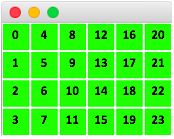
\includegraphics[width=\textwidth]{figures/P5.png}
	\end{subfigure}
	\hspace{0.1\textwidth}
	\begin{subfigure}[h]{0.4\textwidth}
		\centering
		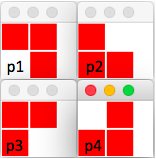
\includegraphics[width=0.75\textwidth]{figures/4p.png}
	\end{subfigure}
	\caption{\label{fig:polyominoes}Polyomino $P$ (à gauche), Polyomino $p$ (à droite), nous autorisons ici toute rotation et réflection. En conséquence, à partir du polyomino $p_1$, nous pouvons en déduire 4 polyominoes. }
\end{figure}
À titre d'exemple, nous allons voir comment carreler un polyomino $P$ de taille $4\times6$ avec un polyomino $p$ de taille $3$ (Figure \ref{fig:polyominoes}). Comme ici la rotation et la réflection des polyominoes sont autorisées, nous avons $S=\{p_1, p_2, p_3, p_4\}$. Nous allons illustrer comment construire des sous-ensembles à partir de $p_2\in S$. Dans cet exemple, il y a 15 positions possibles pour mettre $p_2$ dans $P$. Figure \ref{fig:p2s} nous montre 6 d'entre eux. Les 6 sous-ensembles associés sont $\{0,\,1,\,5\},\,\{8,\,9,\,13\},\,\{16,\,17,\,21\},\,\{2,\,3,\,7\},\,\{10,\,11,\,15\},\,\{18,\,19,\,23\}$. Dans notre exemple, chaque polyomino dans $S$ est associé à 15 sous-ensemble, le problème de carrelage se transforme donc en un problème de la couverture exacte avec 24 colonnes à couvrir et une collection de 60 sous-ensembles. Enfin, Figure \ref{fig:solution} est une solution de notre exemple.

\begin{figure}[t]
	\centering
	\begin{subfigure}[h]{0.35\textwidth}
		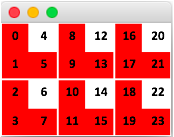
\includegraphics[width=\textwidth]{figures/transition5.png}
		\caption{\label{fig:p2s}Transformer un polyomino en des sous-ensembles}
	\end{subfigure}
	\hspace{0.2\textwidth}
	\begin{subfigure}[h]{0.35\textwidth}
		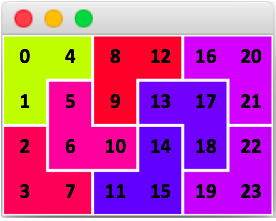
\includegraphics[width=\textwidth]{figures/solution5.png}
		\caption{\label{fig:solution}Une solution}
	\end{subfigure}
	\caption{}
\end{figure}

\subsubsection{N'utiliser chaque polyomino qu'une fois}
Si nous voulons que chaque polyomino soit utilisé exactement une fois, il suffit d'ajouter des colonnes dans les "Dancing Links". Plus précisément, nous pouvons considérer les polyominoes dans la collection $S$ eux-mêmes comme des carrées spéciales et supplémentaires à couvrir, autrement dit, chaque polyomino $p\in S$ correspond à une colonne de plus par rapport à dans la sous-section précédente. Et cette colonne est déterminée seulement par la forme de $p$ qui est indépendante de sa position. Pour illustrer cette idée, revenons sur l'exemple que nous avons évoqué plus haut. Comme les 6 polyominoes rouges dans (Figure \ref{fig:p2s}) ont la même forme, nous pouvons ajouter un élément commun, par exemple 24, dans les 6 sous-ensembles auxquels ils sont associés. Alors, ces 6 sous-ensembles deviennent maintenant $\{0,1,5,24\},\{8,9,13,24\},\{16,17,21,24\},\{2,3,7,24\},\{10,11,15,24\},\{18,19,23,24\}$. Une fois qu'un sous-ensemble contenant 24 est utilisé lors du carrelage, lequel qu'il soit, les autres sous-ensembles contenant 24 ne pourront plus être pris à la suite, ce qui garantit que chaque polyomino est utilisé au plus une fois. D'autre part, si à la fin du carrelage, il existe un polyomino $p\in S$ qui n'est jamais utilisé, alors la colonne appartenant uniquement à $p$ n'est surement pas encore couverte, ce carrelage n'est donc pas une solution de la couverture exacte. Cela garantit que chaque polyomino est utilisé au moins une fois. Nous en déduisons qu'en ajoutant des colonnes de manière intelligente dans les "Dancing Links", nous pouvons assurer que chaque polyomino est utilisé exactement une fois. 

Nous pouvons aussi exiger que chaque polyomino est utilisé au plus une fois. Dans ce cas-là, il faut couper les liaisons entre les colonnes associées aux vraies carrées de $P$ et les colonnes supplémentaires. Vous retrouvez plus de détailles dans notre programme.

\subsection{Question 8}
\subsubsection{Quand $P$ n'est pas un rectangle}
Quand $P$ n'est pas un rectangle, nous pouvons tout de même construire une structure de "Dancing Links" à partir du plus petit rectangle encadrant $P$ en utilisant la même méthode dont nous nous servons dans la Question 7, sauf que cette fois-ci, nous allons pré-couvrir (pré-carreler) les colonnes (carrées) qui sont dans le rectangle mais n'appartiennent pas à $P$. Si nous prenons le polyomino dans (Figure \ref{fig:nonrectangulaire}) comme exemple, il faut pré-couvrir la colonne 0 avant de résoudre le problème de la couverture exacte. Cette méthode n'est pas la plus efficace, mais elle est facile à implémenter.
\begin{figure}
	\centering
	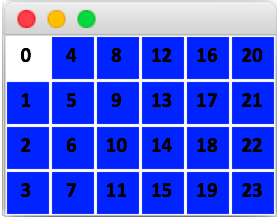
\includegraphics[width=0.45\textwidth]{figures/trou5}
	\caption{\label{fig:nonrectangulaire}Un polyomino non rectangulaire}
\end{figure}

\subsubsection{Réponses aux questions}
Cette sous-section est consacrée à répondre aux questions dans l'énoncé du projet.

\bigskip
\noindent (1) Nous allons d'abord trouver tous les carrelages pour les trois polyominoes dans (Figure \ref{fig:task81}). Les nombres de solutions sont respectivement 303 678 397, 202 195 911 et 140 199 494. (Nous utilisons tous les pentaminoes libres et nous autorisons toutes les opérations isométriques ainsi que la répétition. )
\begin{figure}[h]
	\centering
	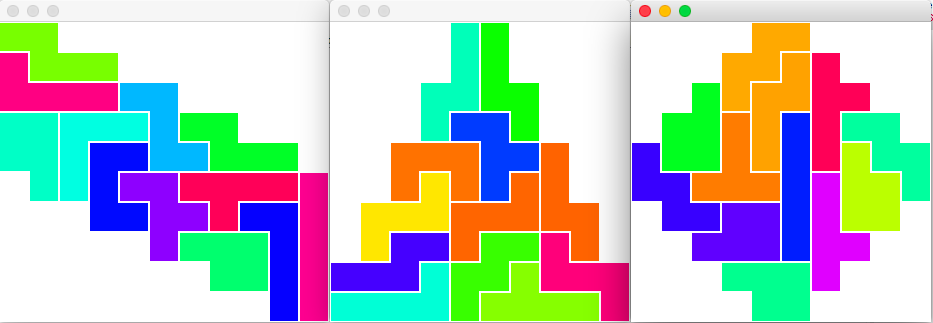
\includegraphics[width=0.9\textwidth]{figures/task8_1}
	\caption{\label{fig:task81}Trouver tous les carrelages de ces trois polyominoes par tous les pentaminoes libres}
\end{figure}

\bigskip
\noindent (2)Étant donné un $n$, nous voulons trouver tous les carrelages possibles d'un rectangle de taille $w \times h$ en utilisant les polyominoes de taille $n$. Pour tester notre programme, nous avons fait trois expériences avec $(w, h, n)=(6,5,6), (6,5,5), (6,6,4)$ (Figure \ref{fig:task8_2}). Ici toute opération isométrique et la répétition sont autorisées.
\begin{figure}[h!]
	\centering
	\begin{subfigure}[h]{0.3\textwidth}
		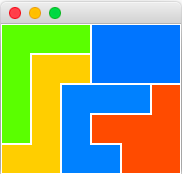
\includegraphics[width=\textwidth]{figures/656.png}
		\caption{}
	\end{subfigure}
	\hspace{0.03\textwidth}
	\begin{subfigure}[h]{0.3\textwidth}
		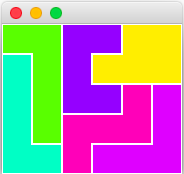
\includegraphics[width=\textwidth]{figures/655.png}
		\caption{}
	\end{subfigure}
	\hspace{0.03\textwidth}
	\begin{subfigure}[h]{0.3\textwidth}
		\centering
		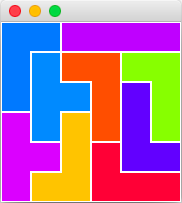
\includegraphics[width=0.85\textwidth]{figures/664.png}
		\caption{}
	\end{subfigure}
	\caption{\label{fig:task8_2} Carrelage d'un rectangle de taille $w \times h$ en utilisant les polyominoes de taille $n$ (a) $(w,h,n)=(6,5,6)$. Le nombre de solutions est 33 344. (b)$(w,h,n)=(6,5,5)$. Le nombre de solutions est 27 950. (c)$(w,h,n)=(6,6,4)$. Le nombre de solutions est 178 935.}
\end{figure}

\bigskip
\noindent (3)Notons $N(n,k)$ tous les polyominoes $P$ de taille $n$ qui peuvent couvrir leurs dilatations $kP$. Alors pour $(n,k)=(8,4)$, nous trouvons que $N(n,k)=10$. Vous voyez quelques exemples dans (Figure \ref{fig:task83})
\begin{figure}[h]
	\centering
	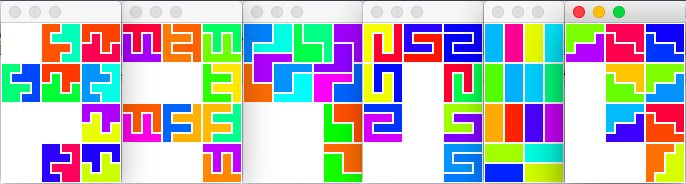
\includegraphics[width=0.9\textwidth]{figures/task8_3}
	\caption{\label{fig:task83} Couvrir sa propre dilatation}
\end{figure}

\subsection{Question 10}
Il y a 6 petites questions dans la Question 10.  Il est difficile de trouver le nombre de solutions pour toutes ces questions. Cependant, nous pouvons répondre aux deux premières questions du carrelage des triangulominoes. Les nombres de solutions sont respectivement 10 et 217 645 229 (65 minutes de calcul, toute opération isométrique et la répétition sont autorisées). Vous trouvez quelques exemples dans (Figure \ref{fig:task10}).

\begin{figure}[h!]
	\centering
	\begin{subfigure}{0.6\textwidth}
		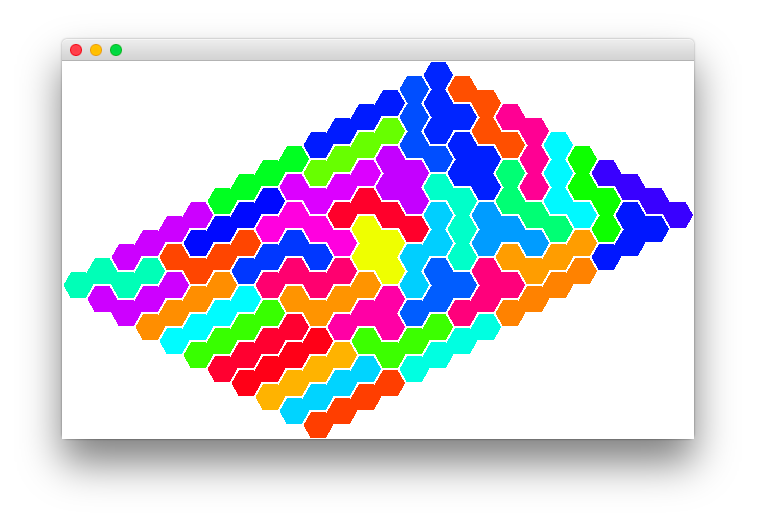
\includegraphics[width=\textwidth]{figures/task10_1.png}
		\caption{}
	\end{subfigure}
	\\
	\begin{subfigure}{0.22\textwidth}
		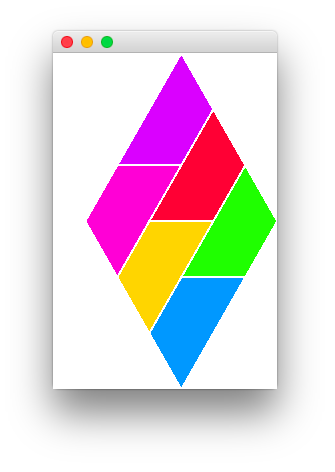
\includegraphics[width=\textwidth]{figures/task10_2.png}
		\caption{}
	\end{subfigure}
	\begin{subfigure}{0.2\textwidth}
		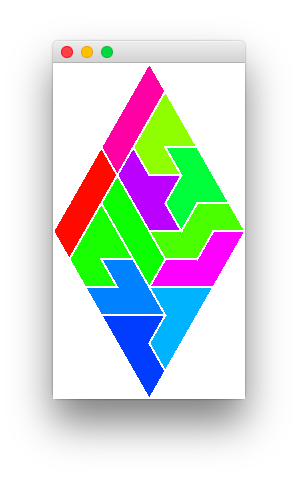
\includegraphics[width=\textwidth]{figures/task10_3.png}
		\caption{}
	\end{subfigure}
	\begin{subfigure}{0.3\textwidth}
		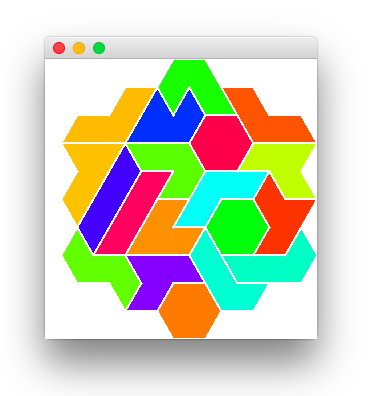
\includegraphics[width=\textwidth]{figures/task10_4.png}
		\caption{}
	\end{subfigure}
	\caption{\label{fig:task10}(a) Carrelage de hexagonamino en utilisant les 44 hexagonaminoes fixés de taille 4. (b) Carrelage de triangulamino en utilisant les 6 triangulaminoes fixés de taille 3. Le nombre de solutions est 10. (c) Carrelage de triangulamino en utilisant les 6 triangulaminoes libres de taille 6. Le nombre de solutions est 217 645 229 (d) Carrelage de triangulamino en utilisant les 19 triangluaminoes à un seul côté de taille 6.}
\end{figure}

\subsection{Question 11}
Pour un problème de sudoku, la taille de $X$ est 324 (Nous avons d'abord 81 cases de la grille de sudoku à couvrir. Il faut 81 $x\in X$ pour représenter ces 81 cases. Cela garantit qu'une case ne sera pas occupée par deux ou plus chiffres. De plus, chaque chiffre entre 1 et 9 ne peut figurer dans une colonne qu'une fois. Il faut donc un $x\in X$ pour marquer qu'un chiffre $i$ figure dans une colonne $j$. Comme nous avons 9 chiffres et 9 colonnes, il nous faut 81 éléments de plus dans $X$. Nous avons le même argument pour les lignes et les petites grilles de taille $3\times3$, ce qui nous faut encore 162 nouveaux éléments dans $X$. Au total, nous avons besoin de 324 éléments dans $X$ ). La taille de la collection $\mathcal{C}$ des sous-ensembles de $X$ est 729 car nous avons 81 cases et 9 chiffres différents.


\section{Conclusion}
\par La NP-complexité du problème de l'énumération de polyominoes et la couverture exacte nous demande de trouver un algorithme et une structure des données assez efficaces qui permettent d'obtenir les résultats pendant une durée accessible et avec un mémoire limité. L'algorithme de Redelmeier pour l'énumération et l'algorithme de \textit{dancing links} ont tous les deux nous montré une efficacité remarquable.
\par Passons de l'énumération de polyominoes à la couverture exacte avec des polyominoes pertinents, nous sommes demandés de stocker les informations des polyominoes que nous trouvons pendant l'énumération. La représentation de tableau binaire est une façons efficace pour à la fois le stockage d'information et les transformations.Accompagné avec cette structure des données, l'algorithme naïf a également une bonne performance grâce à l'efficacité des exploitation par bits pendant l'extension et les transformations des polyominoes.
\par Lorsque nous passons du cas de polyomino au celui de polyiamondes et de polyhex, le squelette des algorithmes pour polyomino restent utils, sauf que nous devons modifier le système de coordonnées pour qu'il soit compatible avec les triangles équilatéraux et les hexagones.

\newpage
\begin{thebibliography}{3}
	\bibitem{redelmeier}
	D.Hugh REDELMEIER.
	"Counting Polyominoes: Yet Another Attack".
	\textit{Discrete Mathematics}, 36(1981):191-203.
	
	\bibitem{dancinglinks}
	Donald Knuth.
	"Dancing Links".
	\textit{Millennial Perspectives in Computer Science}, P159.\textbf{187}. arXiv:cs/0011047v1. Retrieved 2015-11-15.
	
	\bibitem{wikipedia}
	Wikipédia : Polyomino,
	\\\texttt{https://fr.wikipedia.org/wiki/Polyomino}.
	
\end{thebibliography}



\end{document}